\documentclass[10pt, twocolumn]{article}
\usepackage{authblk} % \affil
\usepackage[utf8]{inputenc}
%Gummi|065|=)

\title{\vspace{-2cm}\textbf{Theoretical Guide\\meia noite eu te conto}}
\author{Victor Manuel, Maxwell Oliveira $\&$ Pablo Arruda}
\affil{\textit{Thanks to UFMG - Humuhumunukunukuapua'a}}
\date{}

\usepackage[english]{babel}
\usepackage[utf8]{inputenc}
\usepackage{lscape}
\usepackage[T1]{fontenc}
\usepackage{fancyhdr}
\usepackage{rotating}
\usepackage{ragged2e}
\usepackage[a4paper, landscape, margin=0.8in]{geometry}
\usepackage{blindtext}
\usepackage{amsmath}
\usepackage{relsize}
\usepackage{graphicx}
\usepackage{float}
\usepackage{placeins}
\usepackage{enumitem}
\usepackage{booktabs}
\usepackage{array}
\usepackage{xcolor,colortbl}
\usepackage{tabu}
\usepackage{url}
\usepackage{textcomp}
\usepackage{diagbox}
\usepackage{caption}
\usepackage{amsfonts}
\usepackage{amsmath}
\usepackage{listings} % code
\usepackage{mathtools} % DeclarePairedDelimiter

\usepackage{hyperref}
\hypersetup{
    colorlinks=true,
    linkcolor=blue,
    filecolor=magenta,      
    urlcolor=blue,
}

%color celula da tabela
\usepackage{xcolor,colortbl}

\setlength{\columnseprule}{0.4pt}
\setlength{\columnsep}{3em}
\graphicspath{ {img/} }
\restylefloat{table}

\newcommand{\mc}[2]{\multicolumn{#1}{c}{#2}}
\definecolor{Gray}{gray}{0.85}
\newcolumntype{a}{>{\columncolor{Gray}}c}

\newcommand{\stirlingfirst}[2]{\genfrac{[}{]}{0pt}{}{#1}{#2}}
\newcommand{\stirlingsecond}[2]{\genfrac{\{}{\}}{0pt}{}{#1}{#2}}
\newcommand{\lcm}{\mathrm{lcm}}
\DeclarePairedDelimiter\ceil{\lceil}{\rceil}
\DeclarePairedDelimiter\floor{\lfloor}{\rfloor}

\pagestyle{fancy}

\begin{document}
\maketitle\section{Counting Problems}
\subsection{Burnside's Lemma}

Let $G$ be a group that acts on a set $X$. The Burnside Lemma states that the number of distinct orbits is equal to the average number of points fixed by an element of G.
$$T = \frac{1}{|G|} \sum_{g \in G} |\texttt{fix}(g)|$$
Where a orbit $\texttt{orb}(x)$ is defined as
$$\texttt{orb}(x) = \{y \in X : \exists g \in G \ gx = y \}$$
and $\texttt{fix}(g)$ is the set of elements in $X$ fixed by $g$
$$\texttt{fix}(g) = \{x \in X : gx = x\}$$

\textbf{Example:} With $k$ distinct types of beads how many distinct necklaces of size $n$ can be made? Considering that two necklaces are equal if the rotation of one gives the other.

\begin{center}
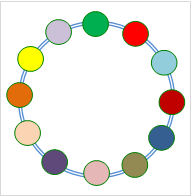
\includegraphics[scale=.6, keepaspectratio]{theoretical/img/Burnside.png}
\end{center}

\begin{align*}
T &= \frac{1}{n+1} \sum_{i=0}^{n}k^{gcd(i, n)} & T &= \frac{1}{n} \sum_{i=0}^{n-1}k^{gcd(i, n)}
\end{align*}

\section{Bitwise}
Turn on bit i \lstinline{x & (1 << i)}\\
Turn off bit i \lstinline{x & (~(1 << i))}\\
\subsection{XOR from 1 to N}

$$
f(n) = \begin{cases}
    n & n \equiv 0\ (\text{mod } 4)\\
    1 & n \equiv 1\ (\text{mod } 4)\\
    n+1 & n \equiv 2\ (\text{mod } 4)\\
    0 & n \equiv 3\ (\text{mod } 4)\\
\end{cases}
$$

\section{C++}
\begin{lstlisting}[language=C++]
template<class T> using min_priority_queue = priority_queue<T, vector<T>, greater<T>>;
\end{lstlisting}

\begin{lstlisting}[language=C++]
string(1, 'a')
\end{lstlisting}
\subsection{Pragma optimize}

\begin{lstlisting}[language=C++]
#pragma GCC optimize("Ofast")
#pragma GCC target("avx,avx2,fma")
\end{lstlisting}
\subsection{Ordered set and multiset}

\begin{lstlisting}[language=C++]
typedef tree<pair<ll, ll>, null_type, less<pair<ll, ll>>, rb_tree_tag, tree_order_statistics_node_update> ordered_set;
\end{lstlisting}

To change to multiset switch equal to less\_equal.
\subsection{Optimized unordered map}

\begin{lstlisting}[language=C++]
mp.reserve(8192);
mp.max_load_factor(0.25);
\end{lstlisting}
\subsection{Interactive Problems}
\begin{lstlisting}[language=C++]
freopen("input.txt", "r", stdin);
freopen("output.txt", "w", stdout);
\end{lstlisting}
\section{Identities}
$$ \sum_{i=1}^{n} i = \dfrac{n(n+1)}{2} \qquad \sum_{i=1}^{n} i^{2} = \frac{n(n+1)(2n+1)}{6} \qquad \sum_{i=1}^{n} i^{3} = \left( \dfrac{n(n + 1)}{2} \right)^2 $$
$$ \sum_{i=1}^{n} \dfrac{1}{i} \approx \log{n} \qquad \sum_{i=0}^{\infty} \dfrac{1}{2^i} = 2 $$

\section{Math}
\subsection{Trigonometry}

\subsection{Logarithm}

$$ \log _{b} mn = \log _{b} m + \log _{b} n \quad\quad log _{b} \dfrac{m}{n} = \log _{b} m - \log _{n} n \quad\quad \log _{b} n^p = p \log _{b} n$$
$$ \log _{b} \sqrt[q]{n} = \dfrac{1}{q} \log _{b} n \quad\quad \log _{b} n = \log _{a} n \log _{b} a \quad\quad b^{\log _{b} k} = k $$
$$ \log _{b} a = \dfrac{\log _{c} a}{\log _{c} b} \quad\quad \log _{b} a = \dfrac{1}{\log _{a} b} \quad\quad \log _{b} a \text{ } \log _{a} c = \log _{b} c $$
$$ \log _{b} 1 = 0 \quad\quad \log _{b} b = 1 $$

\section{Notes}
\begin{itemize}
  \item number of digits in $n!$
  $$ \log _{b} n! = \log _{b} (1 \times 2 \times 3 \times ... \times n) = \log _{b} 1 + \log _{b} 2 + \log _{b} 3 + ... + \log _{b} n $$
\end{itemize}

\section{Geometry}
Fórmulas de geometria plana
\section{Constants}
\begin{lstlisting}[language=C++]
LLINF = 0x3f3f3f3f3f3f3f3fLL
\end{lstlisting}

\begin{lstlisting}[language=C++]
MOD = 998'244'353
\end{lstlisting}

\begin{lstlisting}[language=C++]
PI = acos(-1)
\end{lstlisting}

\section{Number Theory}
$$ (a + b) \text{ mod } m = (a \text{ mod } m + b \text{ mod } m) \text{ mod } m $$
$$ (a - b) \text{ mod } m = (a \text{ mod } m - b \text{ mod } m) \text{ mod } m $$
$$ (a \times b) \text{ mod } m = ((a \text{ mod } m) \times (b \text{ mod } m)) \text{ mod } m $$
$$ a^b \text{ mod } m = (a \text{ mod } m)^b \text{ mod } m $$
$$ a \equiv b \text{ } (\text{mod } m) \iff (b - a) \vert m $$

$$ \gcd(a_1, a_2, a_3, a_4) = \gcd(a_1, \gcd(a_2, \gcd(a_3, a_4))) $$
$$ \lcm(a, b) \times \gcd(a, b) = a \times b $$
$$ \lcm(a, b) = \dfrac{a \times b}{\gcd(a, b)} = \dfrac{a}{\gcd(a,b)} \times b $$
\subsection{Sum of digits of N written in base b}

$$
f(n, b) = \begin{cases}
    n & n < b\\
    f \left( n, \floor*{\dfrac{n}{b}} + (n \mod b) \right) & n \geq b \\
\end{cases}
$$
\subsection{Some Primes}

999999937 $\quad$ 1000000007 $\quad$ 1000000009 $\quad$ 1000000021 $\quad$ 1000000033
$10^{18} - 11 \quad\quad 10^{18} + 3 \quad\quad\quad 2305843009213693951 = 2^{61} - 1$
$998244353 = 119 \times 2^{23} + 1 \quad 10^6+3$
\subsection{Prime counting function - \texorpdfstring{$\pi(x)$}{}}

Expected to have $ \frac{x}{\log{x}} $ primes within $[1, x]$. The prime counting function is asymptotic to $\frac{x}{\log x}$, by the prime number theorem.

\ 

\begin{tabular}{|c|c|c|c|c|c|c|c|c|}
\hline
  \cellcolor{gray!40} x&10&$10^2$&$10^3$&$10^4$&$10^5$&$10^6$&$10^7$&$10^8$\\ \hline
  \cellcolor{gray!40} $\pi(x)$& 4 & 25 & 168 & 1\,229 & 9\,592 & 78\,498 & 664\,579 & 5\,761\,455\\ \hline
\end{tabular}

\ 
\subsection{Number of Divisors}

The number of divisors of $n$ is about $\sqrt[3]{n}$.

\begin{table}[H]
    \centering
    \begin{tabular}{|c|c|c|c|c|c|c|c|c|c|c|c|c|}
        \hline
        \cellcolor{gray!40} $n$ & 6 & 60 & 360 & 5040 & 55440 & 720720 & 4324320 & 21621600 \\
        \hline
        \cellcolor{gray!40} $d(n)$ & 4 & 12 & 24 & 60 & 120 & 240 & 384 & 576 \\
        \hline
    \end{tabular}
\end{table}
\subsection{Large Prime Gaps}
For numbers until $10^9$ the largest gap is 400.\\
For numbers until $10^{18}$ the largest gap is 1500.\\[0.5cm]
\subsection{Fermat's Theorems}

Let P be a prime number and $a$ an integer, then:
$$a^p \equiv a \quad (\text{mod } p)$$
$$a^{p-1} \equiv 1 \quad (\text{mod } p)$$

\textbf{Lemma:} Let $p$ be a prime number and $a$ and $b$ integers, then: 
$$(a+b)^{p} \equiv a^{p} + b^{p} \quad (\text{mod } p)$$

\textbf{Lemma:} Let $p$ be a prime number and $a$ an integer. The inverse of $a$ modulo $p$ is $a^{p-2}$:

$$a^{-1} \equiv a^{p-2} \quad (\text{mod } p)$$
\subsection{Diophantine Equations}

\end{document}
